% -----------------------------------------------
% Template for ISMIR Papers
% 2020 version, based on previous ISMIR templates

% Requirements :
% * 6+n page length maximum
% * 4MB maximum file size
% * Copyright note must appear in the bottom left corner of first page
% * Clearer statement about citing own work in anonymized submission
% (see conference website for additional details)
% -----------------------------------------------

\documentclass{article}
\usepackage[T1]{fontenc} % add special characters (e.g., umlaute)
\usepackage[utf8]{inputenc} % set utf-8 as default input encoding
\usepackage{ismir,amsmath,cite,url}
\usepackage{graphicx}
\usepackage{color}

% Optional: To use hyperref, uncomment the following.
\usepackage[bookmarks=false,hidelinks]{hyperref}
% Mind the bookmarks=false option; bookmarks are incompatible with ismir.sty.

\usepackage{lineno}
%\linenumbers
\newcommand{\carmine}[1]{\textbf{\color{red} Carmine => #1}}
\renewcommand{\baselinestretch}{1}

% Title.
% ------
\title{Neural models for target-based computer-assisted musical orchestration: a preliminary study}

% Note: Please do NOT use \thanks or a \footnote in any of the author markup

% Single address
% To use with only one author or several with the same address
% ---------------
%\oneauthor
% {Names should be omitted for double-blind reviewing}
% {Affiliations should be omitted for double-blind reviewing}

% Two addresses
% --------------
%\twoauthors
%  {First author} {School \\ Department}
%  {Second author} {Company \\ Address}

%% To make customize author list in Creative Common license, uncomment and customize the next line
%  \def\authorname{First Author, Second Author}


% Three addresses
% --------------
%\threeauthors
%  {First Author} {Affiliation1 \\ {\tt author1@ismir.edu}}
%  {Second Author} {\bf Retain these fake authors in\\\bf submission to preserve the formatting}
%  {Third Author} {Affiliation3 \\ {\tt author3@ismir.edu}}

%% To make customize author list in Creative Common license, uncomment and customize the next line
%  \def\authorname{First Author, Second Author, Third Author}

% Four or more addresses
% OR alternative format for large number of co-authors
% ------------
\multauthor
{First author$^1$ \hspace{1cm} Second author$^1$ \hspace{1cm} Third author$^2$} { \bfseries{Fourth author$^3$ \hspace{1cm} Fifth author$^2$}\\
  $^1$ Department of Computer Science, University , Country\\
$^2$ International Laboratories, City, Country\\
$^3$  Company, Address\\
{\tt\small CorrespondenceAuthor@ismir.edu, PossibleOtherAuthor@ismir.edu}
}
\def\authorname{First author, Second author, Third author, Fourth author, Fifth author}


\sloppy % please retain sloppy command for improved formatting

\begin{document}

%
\maketitle
%
\begin{abstract}
In this paper we will do a preliminary exploration on how neural networks can be used for the task of target-based computer-assisted musical orchestration. We will show how it is possible to model this  musical problem as a classification task and we will propose two deep learning models. We will show, first, how they perform as classifiers for musical instrument recognition by comparing them with specific baselines. We will then show how they perform, both qualitatively and quantitatively, in the task of computer-assisted orchestration by comparing them with state-of-the-art systems. Finally, we will highlight benefits and problems of neural approaches for assisted orchestration and we will propose possible future steps.
\end{abstract}
%
\section{Introduction}\label{sec:introduction}

The development of computational tools to assist and inspire the musical composition process constitutes an import research area known as \emph{Computer-Assisted Composition (CAC)} \cite{FerVic2013, Ari2005}. Within CAC, target-based computer-assisted orchestration is an important example of how machine learning can be used for {enhancing} and {assisting} music creativity \cite{Maresz2003}. 

Target-based computer-assisted orchestration can be thought of as the process of searching for the best combinations of sounds in a database of instrumental samples, to match a target sound under a specific similarity metric and specific sets of constraints. A solution to this problem is a set of orchestral scores that represent the mixtures of audio samples in the database, ranked by similarity with the target sound. 
Valid orchestral scores may contain several instruments sounding simultaneously, selected out of a large number of possible combinations of sounds from the database.

\begin{figure}
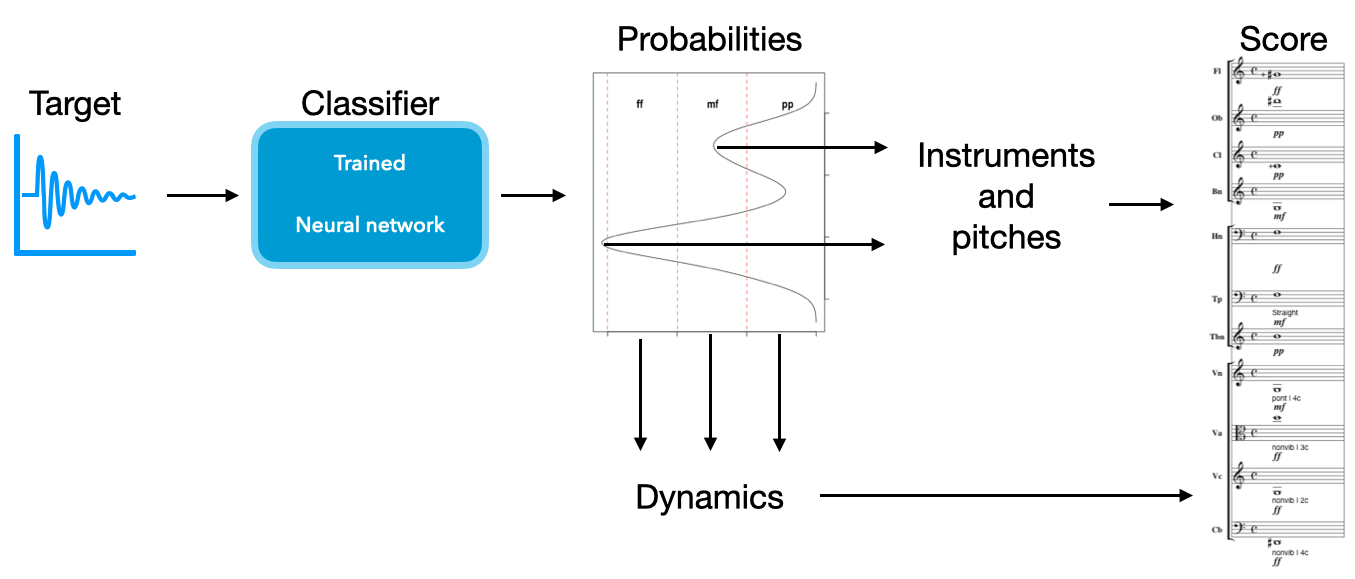
\includegraphics[scale=0.17]{figs/method.png}
\caption{An overview of the proposed method for assisted orchestration with neural models. Instruments and pitches are determined as peaks of the output probability distribution, while the dynamics are computed by quantizing the probabilities. \label{fig:method}}
\end{figure}

The approach studied in \cite{Carpentier2010} consists in finding a good orchestration for any given sound by searching combinations of sounds from a database with a multi-objective optimization heuristics and a constraint solver that are jointly optimized. Both the target sound and the sounds in the database are embedded in a feature space defined by a fixed feature function and each generated combination of sounds is evaluated by using a specific metric. This method has been substantially improved in \cite{Cella18, Cella2020} and is implemented in the \emph{Orchidea} toolbox for assisted orchestration (\url{www.orch-idea.org}), currently considered the state-of-the-art system for assisted orchestration.

In this paper, we try a different approach to this problem by experimenting with deep neural architectures. The main idea is to train a model to classify combinations of real instruments and use it then for orchestration. A typical solution for assisted orchestration is a set of triples \emph{instrument-pitch-dynamics} such as \{\texttt{Flute C6 pp, Bassoon C4 mf, Bassoon G4 ff}\}. By training a neural network with real combinations of instrumental notes, it will acquire the ability to identify the presence of each instrument and its associated pitch by building the appropriate latent representation. Thus, when an unknown target sound is given as input, the network will identify which are the best instruments to match the target sound, and it will be able to  deconstruct a complex mixture of timbres into individual instrument notes.

%\footnote{The dynamics is retrived using the probability distributions generated as output by the network; more details on this will be given in the next sections.}.

This method is motivated by the good results obtained in previous research on musical instruments identification \cite{Benetos07, Kitahara05} and the more recent use of deep neural networks for musical classification \cite{lostanlen16, Bian19}. 

In this paper we do preliminary experiments with two deep architectures: a convolutional neural network (CNN) with a long short-term memory (LSTM) unit in the middle and \emph{ResNet}, a well known residual architecture that already yielded good results for image classification \cite{He15}. We chose to use a CNN because of its success in audio classification \cite{Hershey17} and we decided to include an LSTM unit in it because of its ability to learn long term dependencies in data \cite{Hochreiter97}, which is important given the temporal nature of audio.

After training these models on varying combinations of 10 instruments, we used them for orchestration. More specifically, we orchestrated 15 target sounds by feeding them to the networks and synthesizing a solution from the most likely samples output from the system. We then compared our orchestrations to Orchidea's solutions for the same targets, through both qualitative and quantitative means. For quantitative comparison, we computed a specific distance metric on the FFTs of the target and solution, comparing the distance between Orchidea's solution and the target and our model's solution and the target.

Next sections will be as follows: section \ref{sec:models} will describe the dataset we used for experiments and the models we trained as classifiers, showing the classification results. Sections \ref{sec:orchestration} and \ref{sec:conclusions} will present, respectively, the results of orchestration experiments using the trained models and the conclusions of our preliminary study on neural approaches for target-based computer-assisted orchestration.

The codebase for this paper and some audio examples can be found at: \url{https://github.com/dzluke/DeepOrchestration}.

\section{Neural models}
\label{sec:models}


\begin{figure}
\begin{center}
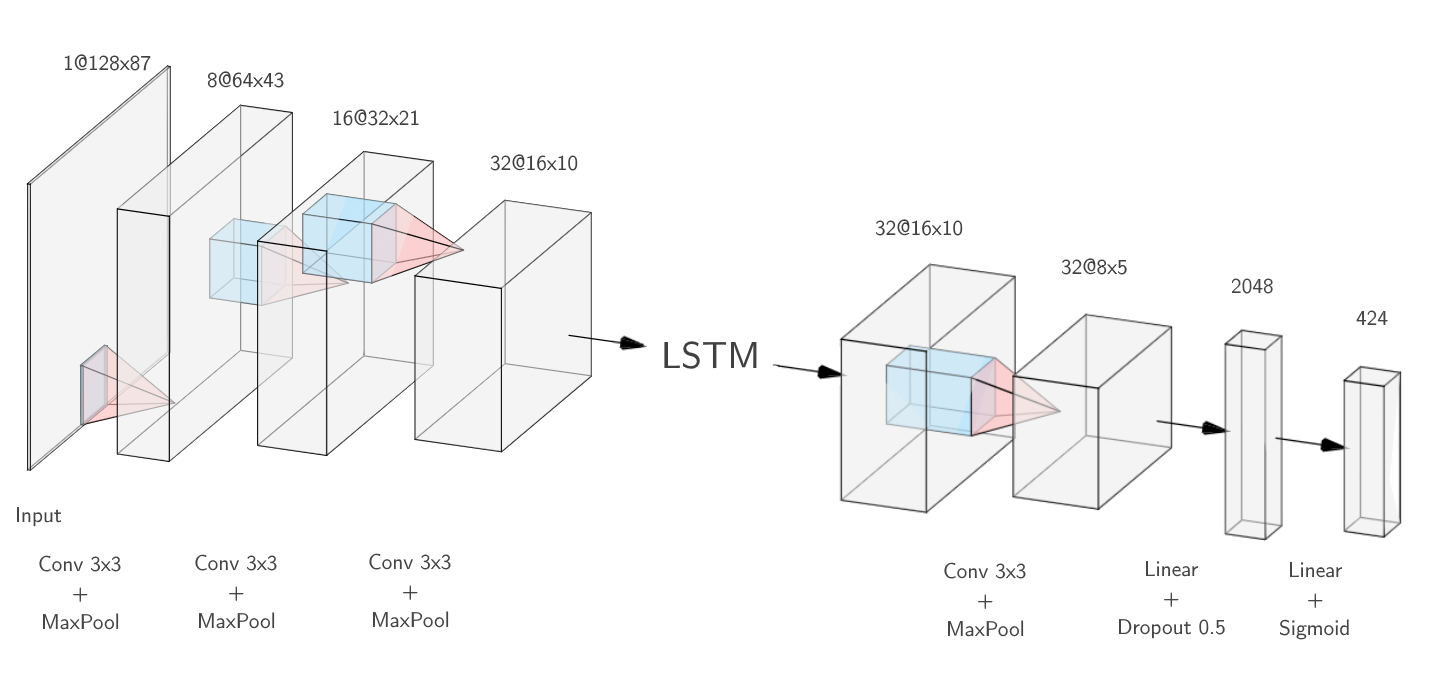
\includegraphics[scale=0.22]{figs/CNN_LSTM_diagram.png}
\caption{Diagram of the CNN with LSTM architecture. \label{cnn_lstm}}
\end{center}
\end{figure}

\subsection{From orchestration to classification}

In this paper, we model assisted orchestration as a classification problem. The general methodology is as follows:
\begin{enumerate}
\item we train specific models to classify the instruments present in combinations of sounds from a database of instrument notes, up to ten simultaneous instruments;
\item we then pick the best classifier and we feed into it an unknown sound to be classified;
\item since the output of the classifier will be in the form of the probability that specific instruments are present in the sound, we use this information to synthesize an orchestration for the target sound;
\item finally, we evaluate the generated orchestration against state-of-the-art systems for computer-assisted orchestrations.
\end{enumerate}

\begin{figure}
\center{
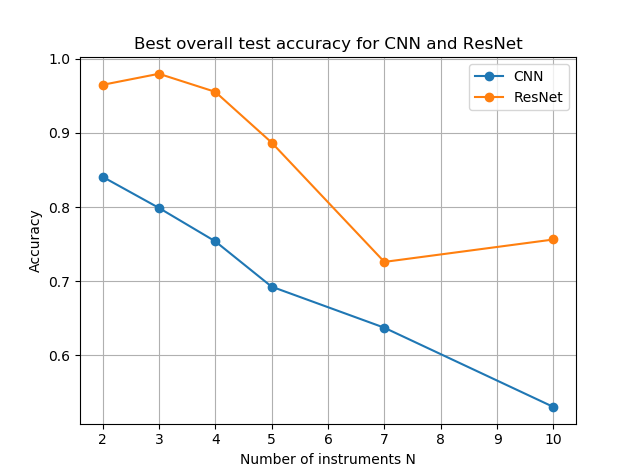
\includegraphics[scale=0.4]{figs/CNN_vs_ResNet.png}}
\caption{Best overall accuracy for CNN with LSTM and ResNet depending on the number of instruments in the combinations used for training. \label{cnn_vs_resnet}}
\end{figure}

In other words, the classifiers learn how to take a complex combination of pitches and timbres and deconstruct it into its original parts.

A complete orchestration solution, however, would normally be made by triples of instrument-pitch-dynamics. It is difficult to frame this problem as classification, since we would need to have a very high number of classes. Moreover, for the nature of the samples we use (a typical sample is in the form \texttt{Flute-C4-pp}, as described in \ref{sec:dataset}), each class would be represented by a single sample. For these reasons, our models have been trained on simplified versions of the original problem and we used different strategies to provide the remaining information needed to generate orchestrations.

In order to have a baseline to compare our classification results and to get a sense on the complexity of the problem, we used various parametric classifiers along with the neural models.

Three baseline classifiers have been trained to recognize either the instrument only for a total of 12 classes (the instruments in TinySOL) or the pair instrument-pitch \emph{class} (a pitch class is the pitch of a note without the corresponding octave, e.g. C, D\#, G, etc.) for a total of 25 classes (we will classifiy combinations of 2 instruments for 12 pitch classes each, plus one extra \emph{trash} class, see section \ref{sec:baseline}).

Two neural classifiers, instead, have been trained on the more complex problem of recognizing instrument-pitch pairs, for a total of 424 classes (i.e. the neural classifiers would classify instruments and pitches with respective octaves, hence 12 instruments for 12 pitch classes and three dynamics; note that not all the samples in TinySOL have all dynamics). We want to point out, however, that this is still a simplified problem compared to assisted orchestration. Even in the case of instrument-pitch pair classification, indeed, we would miss the dynamics of the note. To cope with this problem, in the orchestration phase, we quantize the probability functions generated by the models. When a network is given a target sound as input, it will attempt to apply the same classification rules, outputting a vector of the probabilities of each sample being in the target sound. Since the classes only encode instrument-pitch pairs and since we also need the dynamics, we quantize the probability function generated by the network into three echelons coresponding, respectively, to the dynamic levels \emph{pianissimo}, \emph{mezzoforte} and \emph{fortissimo} (see section \ref{sec:orchestration}). By taking the instruments and pitches that have the highest probability and by using quantized probabilities to retrieve dynamics, a full orchestrated solution can be created.  Figure \ref{fig:method} illustrates the described ideas.

\subsection{Dataset}
\label{sec:dataset}

To create the input data for training the classifiers, we used the \emph{TinySOL} database. TinySOL is a subset of the Studio On Line (SOL) database created by IRCAM \cite{Cella2020b}. TinySOL contains 1,529 samples from 12 instruments. The instruments come from different orchestral families: strings, woodwinds, and brass. Each sample is one instrument playing a single note in the \emph{ordinario} playing style, with one of three dynamics: \textit{pp}, \textit{mf}, or \textit{ff} (for example \texttt{Flute-C4-pp} or \texttt{Clarinet-D5-mf}). 

%The instruments and ranges over which they were recorded are summarized in table \ref{tab:ranges}. 

For a given number of instruments $N$, each input to our models is a combination of $N$ TinySOL samples chosen among an orchestra of 10 instruments. The data is generated in the following way: 

\begin{itemize}
\item $N$ random TinySOL samples are selected, leading to a variety of instruments, pitches, and dynamics; we did not allow the same instrument to be chosen more than three times in order to ensure variety in the mixtures;
\item the chosen samples are combined to be played simultaneously, and the resulting sum is normalized by the number of instruments;
\item the Mel frequency cepstral coefficients (MFCCs) and the Mel spectrogram of the mixture are computed to be used as the input features for the baseline classifiers and the neural classifiers respectively.
\end{itemize}

The resulting combination has a sample rate of $44100$Hz and is padded or trimmed to be exactly 4 seconds long.

The choice of using the Mel spectrogram and MFCCs as input features for classification models is common in music information retrieval \cite{McKinney2003} and can be considered to be an appropriate representation of sound and musical signals. The Mel spectrogram is generated using an FFT hop length of 2048 samples (the window of each FFT was $46$ms wide), and a number of Mel bins equal to 128. Therefore, the Mel features fed to the model were matrices of size $128\times 345$. We used the Librosa package in Python to compute the features; more details on the exact computations can be found in \cite{mcfee15}. The choice of the hop length was made by doing a compromise between the amount of information extracted by each FFT window, and the ability to capture changes in the dynamic, assuming that no change faster than $10$ms would be allowed.

%\begin{table}
%\begin{center}
%\begin{tabular}{|c|c|c|}
%\hline
%\textbf{Instrument} & \textbf{Abbreviation} & \textbf{Range} \\
%\hline
%Violin & Vn & G3-E7\\
%Cello & Vc & C2-C6\\
%Viola & Va & C3-C7\\
%Trumpet C & TpC & F\#3-C6\\
%Trombone & Tbn & A\#0;A\#1-C5\\
%Oboe & Ob & A\#3-A6\\
%Horn & Hn & G1-F5\\
%Flute & Fl & B3-D7\\
%Clarinet Bb & ClBb & D3-G6\\
%Contrabass & Cb & E1-C5\\
%Bass Tuba & BTb & F\#1-F4\\
%Bassoon & Bn & A\#1-D\#5\\
%\hline
%\end{tabular}
%\caption{Table showing the pitch ranges present in the TinySOL database.\label{tab:ranges}}
%\end{center}
%\end{table}

\subsection{Data augmentation}

In order to increase variability in the generated data for the neural models, we also used two methods of data augmentation as described in \cite{Salamon17, Bhardwaj17}; more specifically, we used pitch shifting and partial feature dropout.

The former has been directly applied on the TinySOL samples each time they are selected to generate a new combination. We performed a small pitch shift by reading the samples with different sample rates: a small difference in sample rate will slightly modify the duration and the perceived pitch if played at the normal sample rate. In practice, the sample rates used for this data augmentation were within $5\%$ of the actual $44100$Hz.

The latter was performed on the feature matrix itself of input samples, the Mel spectrogram. We chose random columns and rows of the matrix to zero out. For a given matrix, each column and each row had individually a $1\%$ chance to be set to 0, which yielded an average of $1.28$  columns and $3.45$ rows being zero-ed out. This method of data augmentation aimed to be more resilient to the possible variations in the recording of the instruments.

\subsection{Baselines}
\label{sec:baseline}

In order to get a better sense on the complexity of the problem, we tested three baseline classifiers: support vector machine (SVM), random forest (RF), and K-nearest neighbours (KNN). We used the implementations provided in the \emph{scikit-learn }library for Python \cite{scikit-learn}. More specifically, for SVM we used a non-linear RBF kernel and for RF we set the maximum depth of each tree to be 15.  All of the baseline experiments used 50,000 generated samples with a train-test split of 60/40. Each sample was made by a combination of one to ten instruments and was four seconds in length. 
In this case, differently from the neural models, the features used are the MFCCs of the resulting combination; we chose to use MFCCs for this setting, instead of the Mel spectrogram, to have a lower number of features, that is more manageable by parametric classifiers. We found SVM to have the highest accuracy of the three classifiers across all experiments.

The complete problem of classification of the pairs instrument-pitch has 424 total classes. This problem is very hard for parametric classifiers, so we initially switched to the simpler problem of classifying only the instruments and not the pitch. This had the benefit of both reducing the number of classes and increasing the number of samples per class. We found that SVM was able to very accurately identify the instrument given an input that had only one instrument present; for this case the accuracy was 99.8\%. However, as soon as multiple instruments were present in the input, the accuracy dropped significantly. With two instruments, accuracy was 55.4\%, with three it was 19.6\%. KNN performed significantly worse than SVM, so we did not attempt any further testing with it.

To better approximate our original problem of identifying instrument and pitch, however, we performed experiments in which two instruments were selected and for input data that contained samples from one of those two instruments, both the instrument and pitch \emph{class} of the sample would be classified. The pitch class is the note name without the octave, e.g. C, D\#, G, etc. The input was a combination of two instruments drawn from a possible twelve instruments, and the classifier attempted to identify which instruments were present and for the specified instruments, say Violin and Viola, which pitch classes were present. If another instrument was present in the input combination that was not Violin or Viola, the classifier would simply identify that an instrument that was not one of the two was present. The accuracies from this experiment are outlined in Table \ref{tab:baselines}. Since RF performed worse than SVM in every experiment, we stopped testing with it and used SVM from that point on.

We then performed this same experiment with three instruments having their pitch class identified. Flute, Oboe, and Violin reached an accuracy of 11.1\%, and Bass Tuba, Trumpet, and Trombone was 0.5\%. As we increased the number of instruments whose pitch classes was being identified, the accuracy continued to drop.Indeed, for classifying the pitch class of four instruments (Oboe, French Horn, Violin, and Flute) the accuracy was 2.7\%.

This was still a simplified version of the problem, as we were identifying only the pitch class of a few instruments. However, the parametric classifiers were unable to achieve accurate results as the number of instruments increased. Therefore, we did not attempt, with parametric classifiers, the full setting of the problem in which individual pitches are classified for all instruments. 

\begin{table}
  \begin{center}
    \begin{tabular}{|c|c|c|c|} 
    	  \hline
      \textbf{Instr. 1} & \textbf{Instr. 2} & \textbf{SVM Acc.} & \textbf{RF Acc.}\\
      \hline
      Violin & Flute & 38.8\% & 9.8\% \\
      \hline
      Violin & Trumpet & 33.8\% & 9.1\% \\
      \hline
      Violin & Cello & 34.8\% & 6.3\% \\
      \hline
      Cello & Viola & 32.1\% & 5.8\% \\
      \hline
      Oboe & French Horn & \textbf{39.9\%} & \textbf{17.5\%} \\
      \hline
    \end{tabular}
  \end{center}
  \caption{Comparison of accuracies between SVM and RF. Each data point is a combination of two TinySOL samples, where at least one of the samples is from one of the two instruments specified for that experiment. For the samples drawn from one of the two instruments, the pitch class of that sample is identified. For a sample not from one of the two instruments, the classifier simply attempted to identify that a sample from one of the non-specified instruments was present. In this setting, there are 25 classes: 24 from the 12 pitch classes from 2 instruments, and 1 class that specified whether an instrument that is not one of the two specified is present. \label{tab:baselines}}
\end{table}

In the rest of this section, we will show the classification results of the two neural models. 

\subsection{CNN with LSTM}

The first deep model we trained as a classifier for musical instruments and pitches was a CNN with a LSTM unit. 

%CNNs show good performance on classification problems for their ability to extract spatial features, and have shown success in audio classification \cite{Hershey17}. LSTM units provide a way to learn long term dependencies in the data \cite{Hochreiter97}, which is relevant given the sequential nature of audio.

Our architecture is made of four convolutional layers and two fully connected layers. Each convolutional layer is followed by a BatchNorm layer, a ReLU activation layer and a $2 \times 2$  MaxPool layer with a stride of 2. The kernel size is $3 \times 3$ with a stride of 1 and a padding of 1. The number of filters are 8, 16, 32, and 32.

Following the first three convolutional layers, there is an LSTM layer with 32 outputs. After the LSTM layer, there is a final convolutional layer yielding a tensor of dimensions $32\times 8 \times 21$. We flatten the outputs and feed them into fully a connected layer with Dropout, then another another fully connected layer. Finally, the sigmoid function is applied to the final layer. 

Since each class is independent, we are able to take the sigmoid activation and use binary classification for each class. The model architecture is shown in Figure \ref{cnn_lstm}.

\subsection{ResNet}

The second and more deep model that we trained as classifier was the well known deep residual network \emph{ResNet}. Specifically, we used 18-layer ResNet, which allows information to pass directly from the input to the final layer of each block. Besides, to make the model more suitable to our problem, we decided to reduce the number of parameters and to reset the output channel numbers of each block with 32, 64, 32, 32 respectively.

\subsection{Classification results}

\begin{figure}
\begin{center}
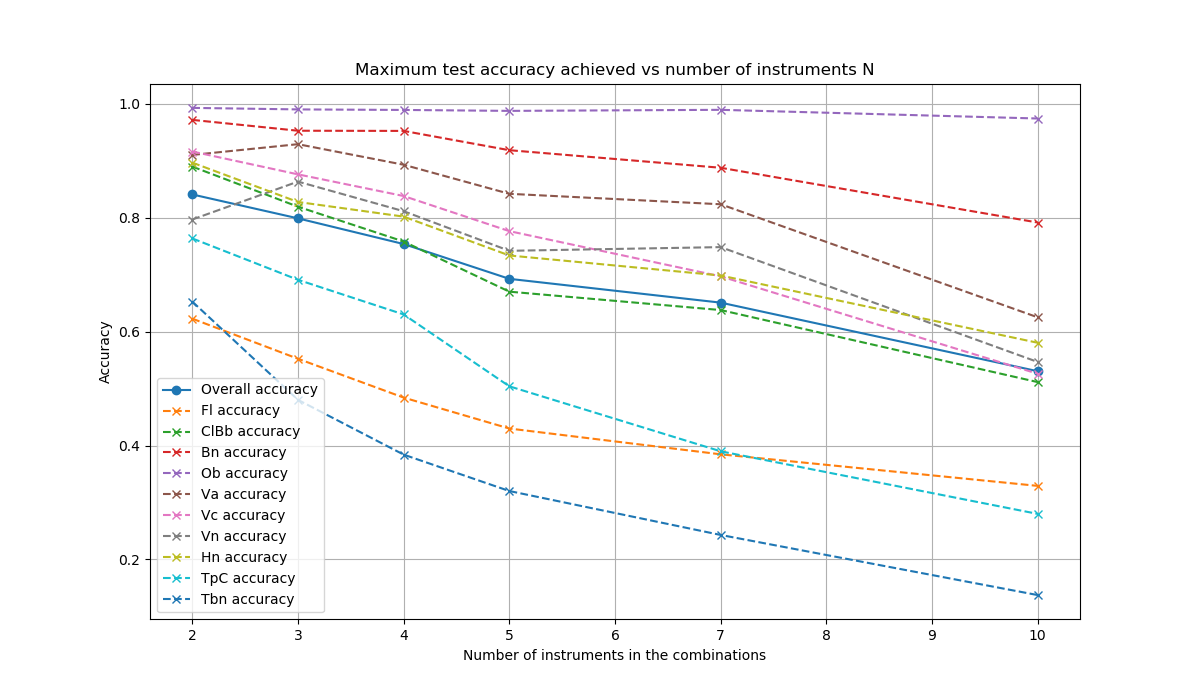
\includegraphics[scale=0.4]{figs/Acc_vs_N_CNN.png}
\caption{Best overall accuracy and for each instrument obtained by the CNN with LSTM depending on the number of instruments in the combinations. \label{best_acc_cnn}}
\end{center}
\end{figure}

During training, the loss function used to optimize the inner parameters of the model was binary cross entropy, as it is the common choice for multiclass multilabel classification frameworks. However, the value of the loss function alone is difficult to interpret. For this reason we created a complementary function $f$ to be used for evaluation only. This function compares a vector of expected outputs $\overline{X}$ with the estimated output from the model $\hat{X}$ by using the following function

\begin{equation}
f(\overline{X}, \hat{X}) = \frac{1}{N}<\overline{X}, M_N(\hat{X})>
\label{eval}
\end{equation}

where

\begin{equation}
M_N(\hat{X})_i = \left\{\begin{array}{ll}
1 \text{ if } i \in I_N(\hat{X})\\
0 \text{ otherwise}
\end{array}\right.
\label{NMax}
\end{equation}
and $I_N(\hat{X})$ is the set of indices containing the $N$ first maximums of the vector $\hat{X}$.

More specifically, the function $M_N(\hat{X})$ takes as an input a vector of probabilities and outputs a vector where only the positions of the $N$ first maxima are set to 1. This new vector would be the orchestration of $N$ instruments given by the model. Thus, the function $f$ simply outputs the proportion of the estimated orchestration that matches the expected one.

Different experiments were made by varying the number $N$ of samples in each mixture. We used an orchestra of 10 instruments containing Horn, Oboe, Violin, Viola, Cello, Flute, Trombone, Bassoon, Trumpet in C and Clarinet in Bb.

Then, for both CNN with LSTM and ResNet, we computed the accuracy on the test sets across epochs, and kept the best one as an indicator of the performance of the models. 
The CNN was trained on 200,000 generated samples over 50 epochs, and ResNet was trained on 400,000 generated samples over 20 epochs. Fig. \ref{cnn_vs_resnet} shows the best overall test accuracy achieved by both models across the number of TinySOL samples $N$ per mixture.\\

ResNet outperforms the CNN regardless of the number of samples used in the combination. This result is consistent with previous research \cite{He15}, as residual networks usually perform well in classification problems.

Fig. \ref{best_acc_cnn} and Fig. \ref{best_acc_resnet} show the maximum accuracy computed using the function $f$ from Eqn. \eqref{eval}. For ResNet, the variance in accuracy is much smaller until $N$ reaches 5, at which point it becomes similar to the CNN. The results on both figures show consistency on the relative accuracy of instruments, which was for us the first step towards the validation of this method. Flute, Trombone and Trumpet yield the worst results for both models. 

While it is not easy to explain these differences in accuracy, we hypothesize this being related to the nature of peculiar spectral and temporal morphology of each instrument. For example, flute notes tend to exhibit a steep spectral rolloff, with most of the energy captured by the first few partials. Moreover, the noisy nature of the transient portions of these note is not well represented by frequency-based descriptions such as Mel spectra. These two factors combined, could make the disentanglement of the flute from the analyzed combination more difficult.

Strings give similar results across both models. An interesting point to notice is the very high accuracy of Oboe on both models. This could indicate that there is an optimal spectral shape that maximizes the probability of being detected in such classification framework.

\begin{figure}
\begin{center}
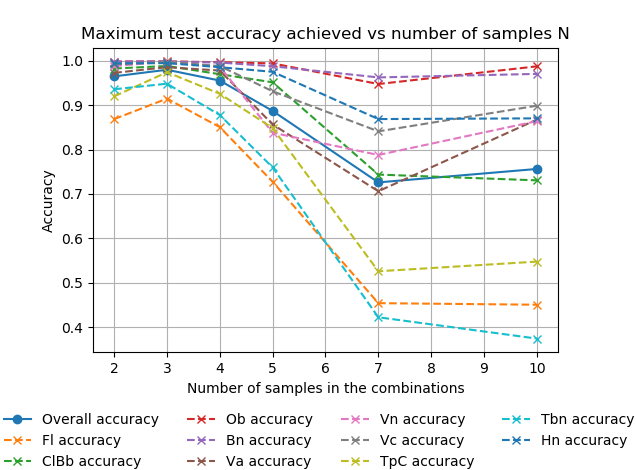
\includegraphics[scale=0.40]{figs/Acc_vs_N_ResNet.png}
\caption{Best overall accuracy and for each instrument obtained by the ResNet depending on the number of instruments in the combinations. \label{best_acc_resnet}}
\end{center}
\end{figure}

\section{Orchestration experiments}
\label{sec:orchestration}

After training the neural models for classification, we finally tested them for the task of target-based computer-assisted orchestration. For this purpose, we decided to use the models trained on combinations of 10 instruments, namely French Horn, Oboe, Violin, Viola, Cello, Flute, Trombone, Bassoon, Trumpet, and Clarinet. Each class, in this model, represents an instrument-pitch pair. 

To orchestrate, a target sound is input to the model, and the 10 classes with the highest probability are extracted. These 10 classes are the instrument-pitch pairs that are most represented in the target, and can be from any combination of the 10 instruments. 

Since we decided not to train our models to classify the dynamics of a sample (despite TinySOL having \emph{pianissimo}, \emph{mezzoforte}, and \emph{fortissimo} recordings), the dynamics are determined by the probability of each sample as output by the model. If the model outputs a probability higher than $0.66$ for a sample, the fortissimo version of the sample is used. If the probability is between $0.33$ and $0.66$, then the mezzoforte version is selected and if it is less than $0.33$ the pianissimo version is used. The idea behind this quantization is that samples that are the most represented in the target should appear as the loudest in the orchestrated solution.

In order to test our models for orchestration, we used 15 targets from the Orchidea distribution. These targets represent a variety of signal types but are mostly static, in the sense that they do not change sensibly over time.

Some of the targets were made of instrumental samples: a sum of oboe and bassoon notes, single bassoon and bass clarinet notes, two multiphonics of bassoon and two symphonic chords. The other targets there are: the recordings of two bells, of a car horn, of a gong, of a screaming voice, of a wind harp, of the attack of a brass instrument and the recording of a boat docking. 

Although the data we trained the model on was fixed to four seconds of audio, the target samples can be of arbitrary length since we adapt the representation to the size of the training data by changing the hop length during the computation of the Mel spectrogram.

\begin{table*}
  \begin{center}
    \label{orch_eval}
    \begin{tabular}{|c|c|c|c|c|c|c|c|c|c}
     \hline
      \textbf{Model} & \textbf{Ob + Bn} & \textbf{Bn} & \textbf{Bass cl.} & \textbf{Bell 1} & \textbf{Bell 2} & \textbf{Multiph. 1} & \textbf{Car horn} & \textbf{Boat} $\ldots$ \\
      \hline
      CNN with LSTM & 0.17 & 0.28 & 0.70 & 0.55 & 0.26 & \textbf{1.10} & 0.68 & \textbf{1.12} $\ldots$  \\
      \hline
      ResNet & 0.34 & 0.50 & 0.48 & 0.59 & 0.45 & 0.90 & 0.49 & \textbf{1.16} $\ldots$ \\
      \hline
      \hline
      \textbf{$\ldots$} & \textbf{Wind harp} & \textbf{Chord 1} & \textbf{Multiph. 2} & \textbf{Chord 2} & \textbf{Gong} & \textbf{Scream} & \textbf{Brass} & \textbf{Average}  \\
      \hline
      $\ldots$ & 0.55 & 0.79 & 0.70 & 0.57 & 0.73 & \textbf{1.14} & 0.79 & 0.71\\
      \hline
      $\ldots$  & 0.61 & 0.86 & 0.51 & 0.37 & 0.71 & \textbf{1.03} & \textbf{1.05} & 0.66 \\
      \hline
    \end{tabular}
  \end{center}
  \caption{Quantitative comparison of orchestrations as ratios to Orchidea. Eqn. \eqref{distance} was used with $\lambda_1 = 0.5$ and $\lambda_2 = 10$ to compute distances between orchestrations and targets. What is shown is the ratio between the distance calculated and Orchidea's distance for the same target. A value less than 1 means that the model performed worse (i.e. had a larger distance), and a value greater than 1 means the model performed better than Orchidea. The last column shows the ratio of the average distances for the model across all targets.}
\end{table*}

\subsection{Evaluation}

We evaluated our orchestrations both qualitatively and quantitatively by comparing our solutions to the solutions generated by Orchidea, the state-of-the-art system for computer-assisted orchestration. 

Orchidea implements many advanced features that are not supported by our models. For example, it is able to apply symbolic constraints to the search, hence allowing only specific instrumental combinations or playing styles. It is also able to reduce the search space by applying harmonic analysis on the target sound.
The dominant harmonic partials of the target are identified, and the search space is limited to only include samples of those pitches. For example, if the target is a recording of an instrument playing a C4, then the partials identified may be C4, C5, G5, and E6. The model would then only consider samples of these pitches to be used in the solution. This leads to a solution whose harmonics are much closer to the target, which is an important part of aural similarity.
Orchidea's solutions, moreover, can use any number of instruments included in the orchestra specified by the user, thus having variable-sized orchestrations from a single instrument to the whole set (this property is called \emph{sparsity} of the solution).

In order to have a more fair comparison, we did not allow Orchidea to use any of the advanced features: we did not apply any symbolic constraints or harmonic analysis and we forced it forced to use all 10 instruments in each solution. This creates a more fair comparison, since our models are unable to create constrained or sparse solutions.

Qualitative evaluation was done through an acoustic inspection of the solution, paying close attention to timbre and pitch. For targets that had harmonic content, it was noted if the partials present in the target were also represented in the orchestrated solution. For example, one of the samples of a bell had partials that loosely represented a C minor chord, so we checked if the orchestration contained the notes of the chord. If a target had specific notes, we identified if the note or its partials were present. For example there is target of an Oboe playing an A4 and a Bassoon playing a C\#3, the solution from ResNet contained the partials of the Bassoon's note: C\#3, G\#4, C\#5, and E6 were all included on various instruments in the solution.

For quantitative evaluation, we used the distance metric defined in Eqn. \eqref{distance} to calculate differences in timbre between targets and solutions. This metric is proposed in \cite{Cella2020} as part of the cost function used in Orchidea during the optimization. The equation takes in the full FFT of the target $x$ and full FFT of the solution $\hat{x}$. Then for each bin $k$ of the FFT, it calculates the absolute difference between the values. The differing values of $\lambda_1$ and $\lambda_2$ allow the metric to penalize the solution in different ways. 

In the first summation, $\lambda_1$ is multiplied by all the distances calculated when there was more energy in the target than the solution, since $\delta_{k1} = 1$ only when $x_k \ge \tilde{x}_k$. Similarly in the second summation, $\lambda_2$ is multiplied by all the distances when the solution provided more energy to a frequency than the target. Therefore, the relation between $\lambda_1$ and $\lambda_2$ determines whether a solution is penalized more for undershooting or overshooting the target.

We calculated the distance between the target samples and our orchestrated solutions. We then orchestrated the same targets with Orchidea and calculated the distance for Orchidea's solutions. A comparison of these results is in Table \ref{orch_eval}.

\begin{equation}\label{distance}
d(x, \tilde{x}) =\lambda_1 \sum_k \delta_{k1}(x_k - \tilde{x}_k) + \lambda_2 \sum_k \delta_{k2}|x_k - \tilde{x	}_k| \\
\end{equation}
where 
$
\delta_{k1} = 
\begin{cases}
1, \text{if   } x_k \ge \tilde{x}_k \\
0, \text{otherwise}
\end{cases} 
$, $
\delta_{k2} = 
\begin{cases}
1, \text{if   } x_k < \tilde{x}_k \\
0, \text{otherwise}
\end{cases}.
$\\

While our model is not able to outperform Orchidea, it shows consistent results. We find that the CNN and ResNet give similar accuracies during training, but perform differently when tasked with orchestrating targets. Overall, CNN seems to better emulate the timbre in its orchestrations, where ResNet is better for recreating the harmonic content of the target. 

\section{Conclusions}
\label{sec:conclusions}

Target-based computer-assisted orchestration through deep learning models seems a promising path, thanks to the ability of deep networks to classify individual instruments and pitches out of dense combinations of samples. This work, however, represents only a preliminary study of the potential of these methods for the task of assisted orchestration. 

The first natural extension would be to support sparsity in our models. Our current models, indeed, orchestrate all targets using a constant number of instruments and it is not able to drop specific instruments from the solution. This does not take into account the density of different targets. Sparse solutions, in which the model decides how many samples should be used to best represent the target, would allow a small number of samples to be used for sonically sparse sounds and many to be used for sonically dense sounds. This would generate more meaningful orchestrations that would compare more favourably to the state of the art.

Another important extension would be to create a more powerful embedding spaces for the target and combinations. In \cite{Gillick19} the authors propose to use LSTM-based models to predict the embedding features for the combinations used during the optimisation process in assisted orchestration. We believe that by combining their prediction model with our classification models could generate more faithful representations and improve the overall quality of generated orchestrations.

%\subsection{Interpreting the Latent Space}
%
%After training the CNN with LSTM for $N=10$ samples per combination, it is possible to visualize the filters applied to the input layer after layer. Figs. \ref{latent0}-\ref{latent5} show the successive outputs of each layer of the convolutional network. \carmine{I put here all the intermediary features of the CNN with LSTM. I don't find any particular conclusion other than saying that LSTM seems to focus more on vertical components rather than horizontal, ie time over frequency}
%
%\begin{figure}
%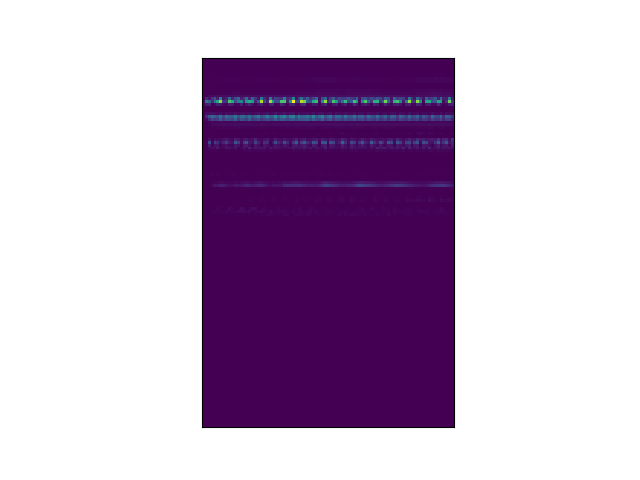
\includegraphics[scale=0.5]{figs/latent_space_layer0.png}
%\caption{Initial feature matrix used as input of the model \label{latent0}}
%\end{figure}
%
%\begin{figure}
%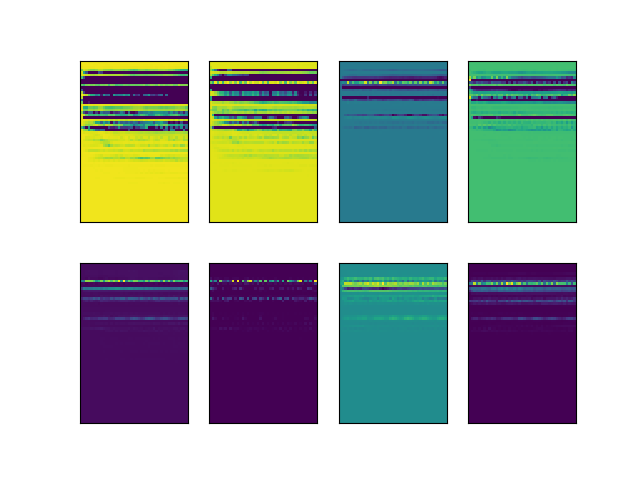
\includegraphics[scale=0.5]{figs/latent_space_layer1.png}
%\caption{Intermediary features after the first convolutional layer of the CNN with LSTM. \label{latent1}}
%\end{figure}
%
%\begin{figure}
%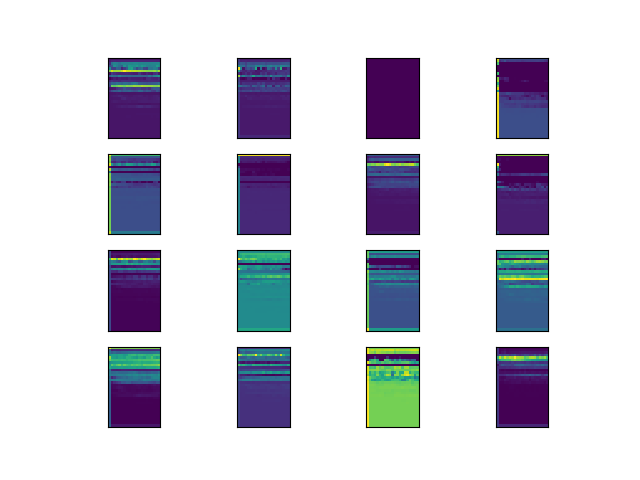
\includegraphics[scale=0.5]{figs/latent_space_layer2.png}
%\caption{Intermediary features after the second convolutional layer of the CNN with LSTM. \label{latent2}}
%\end{figure}
%
%\begin{figure}
%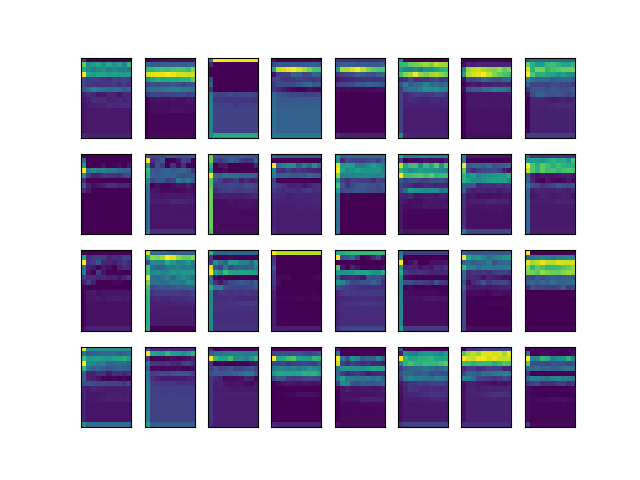
\includegraphics[scale=0.5]{figs/latent_space_layer3.png}
%\caption{Intermediary features after the third convolutional layer of the CNN with LSTM. \label{latent3}}
%\end{figure}
%
%\begin{figure}
%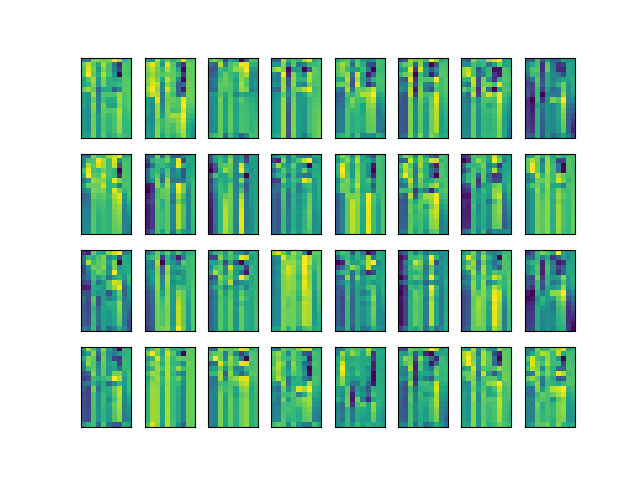
\includegraphics[scale=0.5]{figs/latent_space_layer4.png}
%\caption{Intermediary features after the LSTM layer. \label{latent4}}
%\end{figure}
%
%\begin{figure}
%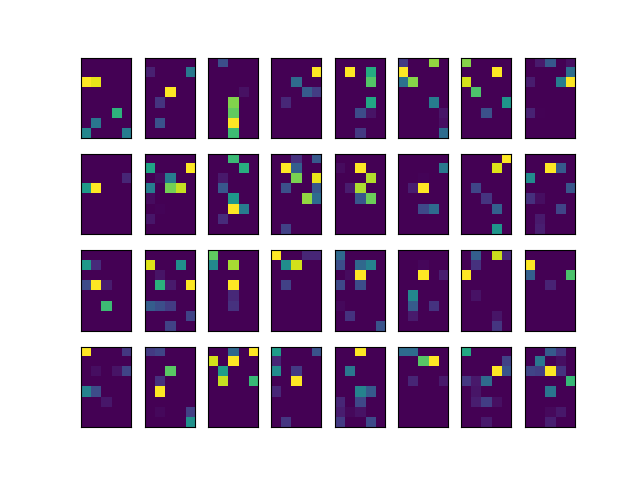
\includegraphics[scale=0.5]{figs/latent_space_layer5.png}
%\caption{Intermediary features after final convolutional layer of the CNN with LSTM. \label{latent5}}
%\end{figure}

\iffalse
\begin{figure}
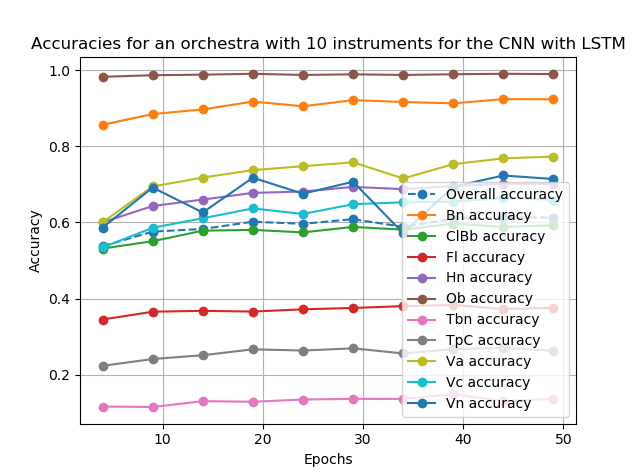
\includegraphics[scale=0.6]{figs/CNN10.png}
\end{figure}
\fi

% For bibtex users:
%\bibliography{paper}

\begin{thebibliography}{99}

\bibitem{FerVic2013} Jose David Fern\'andez and Francisco Vico. {AI Methods in Algorithmic Composition: A Comprehensive Survey}. Journal of Artificial Intelligence Research, vol.48, pp. 513--582, 2013.

\bibitem{Ari2005} Christopher Ariza, {Navigating the landscape of computer aided algorithmic composition systems: A definition, seven descriptors, and a lexicon of systems and research}. In Proceedings of the International Computer Music Conference, 2005.

\bibitem{Maresz2003}
Yan Maresz, {On Computer-Assisted Orchestration}. Contemporary Music Review, vol. 32, n. 1, pg. 99-109, Routledge, 2013.

\bibitem{Carpentier2010}
Gr\'egoire Carpentier, Damien Tardieu, Jonathan Harvey, G\'erard Assayag and Emmanuel Saint-James. {Predicting Timbre Features of Instrument Sound Combinations: Application to Automatic Orchestration}, Journal of New Music Research, vol. 39, n. 1, pg. 47-61, Routlegde, 2010.


\bibitem{Benetos07}
Emmanouil Benetos, Margarita Kotti, and Constantine Kotropoulos.
\newblock Large scale musical instrument identification.
\newblock Sound and Music Computing Conference, Greece, 2007.

\bibitem{Bhardwaj17}
Siddharth Bhardwaj.
\newblock Audio data augmentation with respect to musical instrument
  recognition.
\newblock Master's thesis, 2017.

\bibitem{Bian19}
Wenhao Bian, Jie Wang, Bojin Zhuang, Shaojun~Wang Jiankui~Yang, and Jing Xiao.
\newblock Audio-based music classification with densenet and data augmentation.
\newblock arXiv preprint, https://arxiv.org/abs/1906.11620v1, 2019.

\bibitem{Cella2020}
Carmine-Emanuele Cella.
\newblock Orchidea: a comprehensive framework for target-based assisted orchestration.
\newblock In preparation; available on request from the author, 2020.

\bibitem{Cella2020b}
Carmine-Emanuele Cella, Daniele Ghisi, Vincent Lostanlen, Fabi\'en Levy, Yan Maresz and Joshua Fineberg.
\newblock OrchideaSOL: a dataset of extended instrumental techniques for computer-aided orchestration.
\newblock ICMC (under review), 2020.

\bibitem{Chetry05}
Nicolas Chetry, Mike Davies, and Mark Sandler.
\newblock Musical instrument identification using LSF and K-means.
\newblock Audio Engineering Society Convention 118, 2005.

\bibitem{He15}
Kaiming He, Xiangyu Zhang, Shaoqing Ren, and Jian Sun.
\newblock Deep residual learning for image recognition.
\newblock arXiv preprint, https://arxiv.org/abs/1512.03385, 2015.

\bibitem{Hershey17}
Shawn Hershey, Sourish Chaudhuri, Daniel P.~W. Ellis, Jort~F. Gemmeke, Aren
  Jansen, R.~Channing Moore, Manoj Plakal, Devin Platt, Rif~A. Saurous, Bryan
  Seybold, Malcolm Slaney, Ron~J. Weiss, and Kevin Wilson.
\newblock CNN architectures for large-scale audio classification.
\newblock IEEE International Conference on Acoustics, Speech and Signal Processing (ICASSP), 2017.

\bibitem{Hochreiter97}
Sepp Hochreiter and J\"{u}rgen Schmidhuber.
\newblock Long short-term memory.
\newblock {\em Neural Comput.}, 9(8):1735–1780, November 1997.

\bibitem{Kitahara05}
Tetsuro Kitahara, Masataka Goto, and Hiroshi~G. Okuno.
\newblock Pitch-dependent identification of musical instrument sounds.
\newblock Applied Intelligence 23, 267–275, Springer, 2005.

\bibitem{lostanlen16}
Vincent Lostanlen and Carmine-Emanuele Cella.
\newblock Deep convolutional networks on the pitch spiral for musical
  instrument recognition. ISMIR, 2016.

\bibitem{mcfee15}
Brian McFee, Colin Raffel, Dawen Liang, Daniel~P.W. Ellis, Matt McVicar, Eric
  Battenberg, and Oriol Nieto.
\newblock librosa: Audio and music signal analysis in python.
\newblock {P}roceedings of the 14th {P}ython in {S}cience {C}onference, 2015.

\bibitem{scikit-learn}
Fabian Pedregosa, Ga\"el Varoquaux, Alexandre
Gramfort, Vincent Michel, Bertrand Thirion, Olivier
Grisel, Mathieu Blondel, Peter Prettenhofer, Ron
Weiss, Vincent Dubourg, Jake Vanderplas, Alexandre
Passos, David Cournapeau, Matthieu Brucher,
Matthieu Perrot, \'Edouard Duchesnay.
\newblock Scikit-learn: Machine learning in {P}ython.
\newblock {\em Journal of Machine Learning Research}, 12:2825--2830, 2011.

\bibitem{Salamon17}
Justin Salamon and Juan~Pablo Bello.
\newblock Deep convolutional neural networks and data augmentation for
  environmental sound classification.
\newblock {\em IEEE Signal Processing Letters}, 24(3):279–283, Mar 2017.

\bibitem{McKinney2003}
Martin F. McKinney and Jeroen Breebaart.
\newblock Features for Audio and Music Classification.
\newblock ISMIR, 2003.

\bibitem{Cella18}
Carmine-Emanuele Cella and Philippe Esling, {Open-source modular toolbox for computer-aided orchestration}, Proc. of the Timbre conference, Montreal, Canada, 2018.

\bibitem{Gillick19}
Jon Gillick, Carmine-Emanuele Cella and David Bamman. {Estimating Unobserved Audio Features for Target-Based Orchestration}, ISMIR, 2019.

\end{thebibliography}

\end{document}

